\section{Coin Collector Robot}

\textbf{(a)}

The robot has constant unit speed in the \(y\)-direction, so
\[
    y(t)=t
\]
In the \(x\)-direction, the mass is one, so the acceleration is the
applied force. With initial position and velocity equal to zero,
\[
    x(t)=\int_0^t (t-\tau)f(\tau)\,d\tau
\]
For the first few integer times, this gives
\[
\begin{aligned}
    x(1)
        &=\int_0^1 (1-\tau)f_1\,d\tau
          =\frac{1}{2}f_1\\
    x(2)
        &=\int_0^2 (2-\tau)f_1\,d\tau
          =2f_1\\
    x(3)
        &=\int_0^2 (3-\tau)f_1\,d\tau
          +\int_2^3 (3-\tau)f_2\,d\tau
          =4f_1+\frac{1}{2}f_2\\
    x(4)
        &=\int_0^2 (4-\tau)f_1\,d\tau
          +\int_2^4 (4-\tau)f_2\,d\tau
          =6f_1+2f_2
\end{aligned}
\]
The same pattern extends to all integer times. Since \(f_j\) is applied for
\[
    2j-2\leq t<2j
\]
define the matrix \(A\in\mathbb{R}^{2n\times n}\) by
\[
    A_{tj}=
    \begin{cases}
        0, & t\leq 2j-2,\\[3pt]
        \frac{1}{2}(t-(2j-2))^2, & 2j-2<t<2j,\\[3pt]
        2(t-2j+1), & t\geq 2j
    \end{cases}
\]
Then the \(x\)-coordinate at integer time \(t\) is
\[
    x(t)=\sum_{j=1}^n A_{tj}f_j
\]
Finally, the robot coordinates at integer time \(t\) are
\[
    \left(\sum_{j=1}^n A_{tj}f_j,\ t\right)
\]

\textbf{(b)}

Since \(y_i=i\), the robot can collect coin \(i\) only at time \(t=i\).
Using the matrix \(A\) from part (a), if
\(x_{\mathrm{coin}}\in\mathbb{R}^{2n}\) is the vector of coin
\(x\)-coordinates, then collecting all coins requires
\[
    Af=x_{\mathrm{coin}}
\]
So the desired coin vector must lie in the range of \(A\):
\[
    x_{\mathrm{coin}}\in\operatorname{range}(A)
\]
This can be checked using least squares, and checking the error is zero:
\[
\begin{aligned}
    \hat f&=\operatorname*{arg\,min}_g\|Ag-x_{\mathrm{coin}}\|_2\\
    r&=A\hat f-x_{\mathrm{coin}}
\end{aligned}
\]
If the residual is nonzero, no input force vector can collect that set of coins exactly.

\textbf{(c)}

\[
    n=6,\qquad
    x_{\mathrm{coin}}=
    \left[\begin{array}{rrrrrrrrrrrr}
        0.5 & 2 & 2 & -2 & -4.5 & 0 & 13 & -4 & -6 & 12 & 22.5 & -2
    \end{array}
    \right]^\top
\]
These are the horizontal coordinates of the \(12\) coins. Collecting
every coin requires
\(
    Af=x_{\mathrm{coin}}
\)
where \(f=(f_1,\ldots,f_6)\).

From the first coin,
\[
    \frac{1}{2}f_1=0.5\Rightarrow f_1=1
\]
Coin \(3\) gives
\[
    4f_1+\frac{1}{2}f_2=2 \Rightarrow 4+\frac{1}{2}f_2=2\Rightarrow f_2=-4
\]
Coin \(5\) gives
so
\[
    8f_1+4f_2+\frac{1}{2}f_3=-4.5 \Rightarrow 8-16+\frac{1}{2}f_3=-4.5\Rightarrow f_3=7
\]
Coin \(7\) requires
\[
    12f_1+8f_2+4f_3+\frac{1}{2}f_4=13 \Rightarrow
    12-32+28+\frac{1}{2}f_4=13\Rightarrow f_4=10
\]
Coin \(8\) requires
\[
    14f_1+10f_2+6f_3+2f_4=-4 \Rightarrow
    14-40+42+2f_4=-4\Rightarrow f_4=-10
\]

Collecting coin \(7\) requires \(f_4=10\), while collecting coin
\(8\) requires \(f_4=-10\). This is impossible, so the robot can't collect all coins.

\textbf{(d)}

For each coin, let's remove that coin's
equation from the system and solve for the force vector using the
remaining equations. Then I check how far the resulting robot positions
are from the remaining coin positions. If the largest error is essentially
zero, then that choice works.

\textbf{(e)}

\begin{figure}[H]
    \centering
    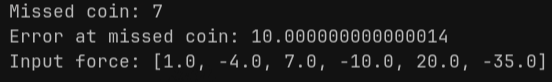
\includegraphics[width=0.8\textwidth]{img/2e.png}
    % \caption{Missed coin, error on missed coin and force}
\end{figure}

\begin{figure}[H]
    \centering
    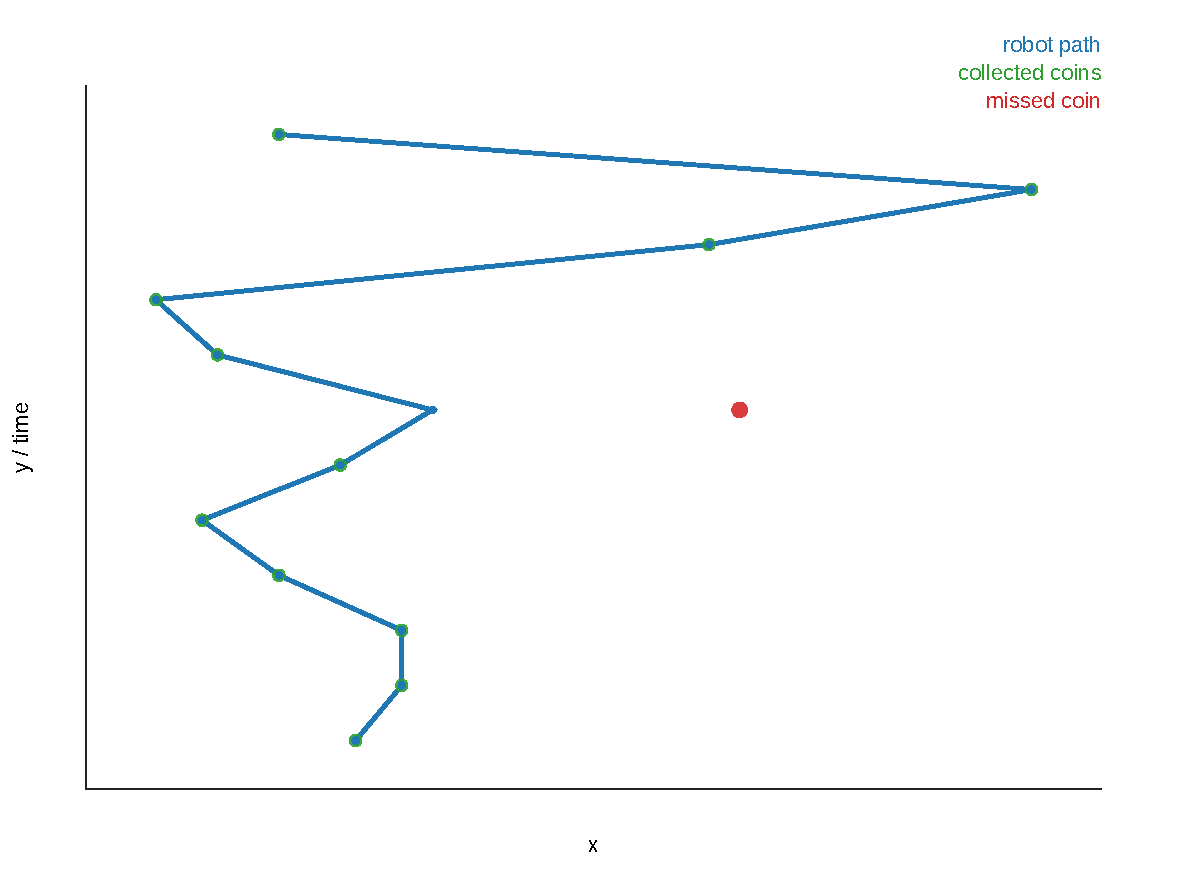
\includegraphics[width=0.82\textwidth]{img/p2_robot_path.pdf}
    \caption{Coin locations and robot positions}
\end{figure}

\textbf{Code}

\begin{lstlisting}
using LinearAlgebra

A = zeros(2n, n)
for t in 1:(2n), j in 1:n
    interval_start = 2j - 2
    interval_end = 2j

    if t <= interval_start
        A[t, j] = 0.0
    elseif t < interval_end
        A[t, j] = 0.5 * (t - interval_start)^2
    else
        A[t, j] = 2 * (t - 2j + 1)
    end
end

missed_coin = nothing
best_f = nothing
best_residual = nothing
missed_error = nothing
tol = 1e-8

for miss in 1:(2n)
    rows = [i for i in 1:(2n) if i != miss]
    f = A[rows, :] \ coin_x[rows]

    residual = norm(A[rows, :] * f - coin_x[rows], Inf)

    if residual <= tol
        missed_coin = miss
        best_f = f
        best_residual = residual
        missed_error = abs((A * f - coin_x)[miss])
        break
    end
end

println("Missed coin: ", missed_coin)
println("Error at missed coin: ", missed_error)
println("Input force: ", round.(best_f; digits=4))
\end{lstlisting}
